\section{Processing manager}

Processing manager is the major component in the processing of a HLASM source file. It decides which stream of statements is about to be processed and assigns it to the correct processor. It contains components responsible for instruction interpretation as well as instruction format validation. 

\begin{figure}
	\centering
	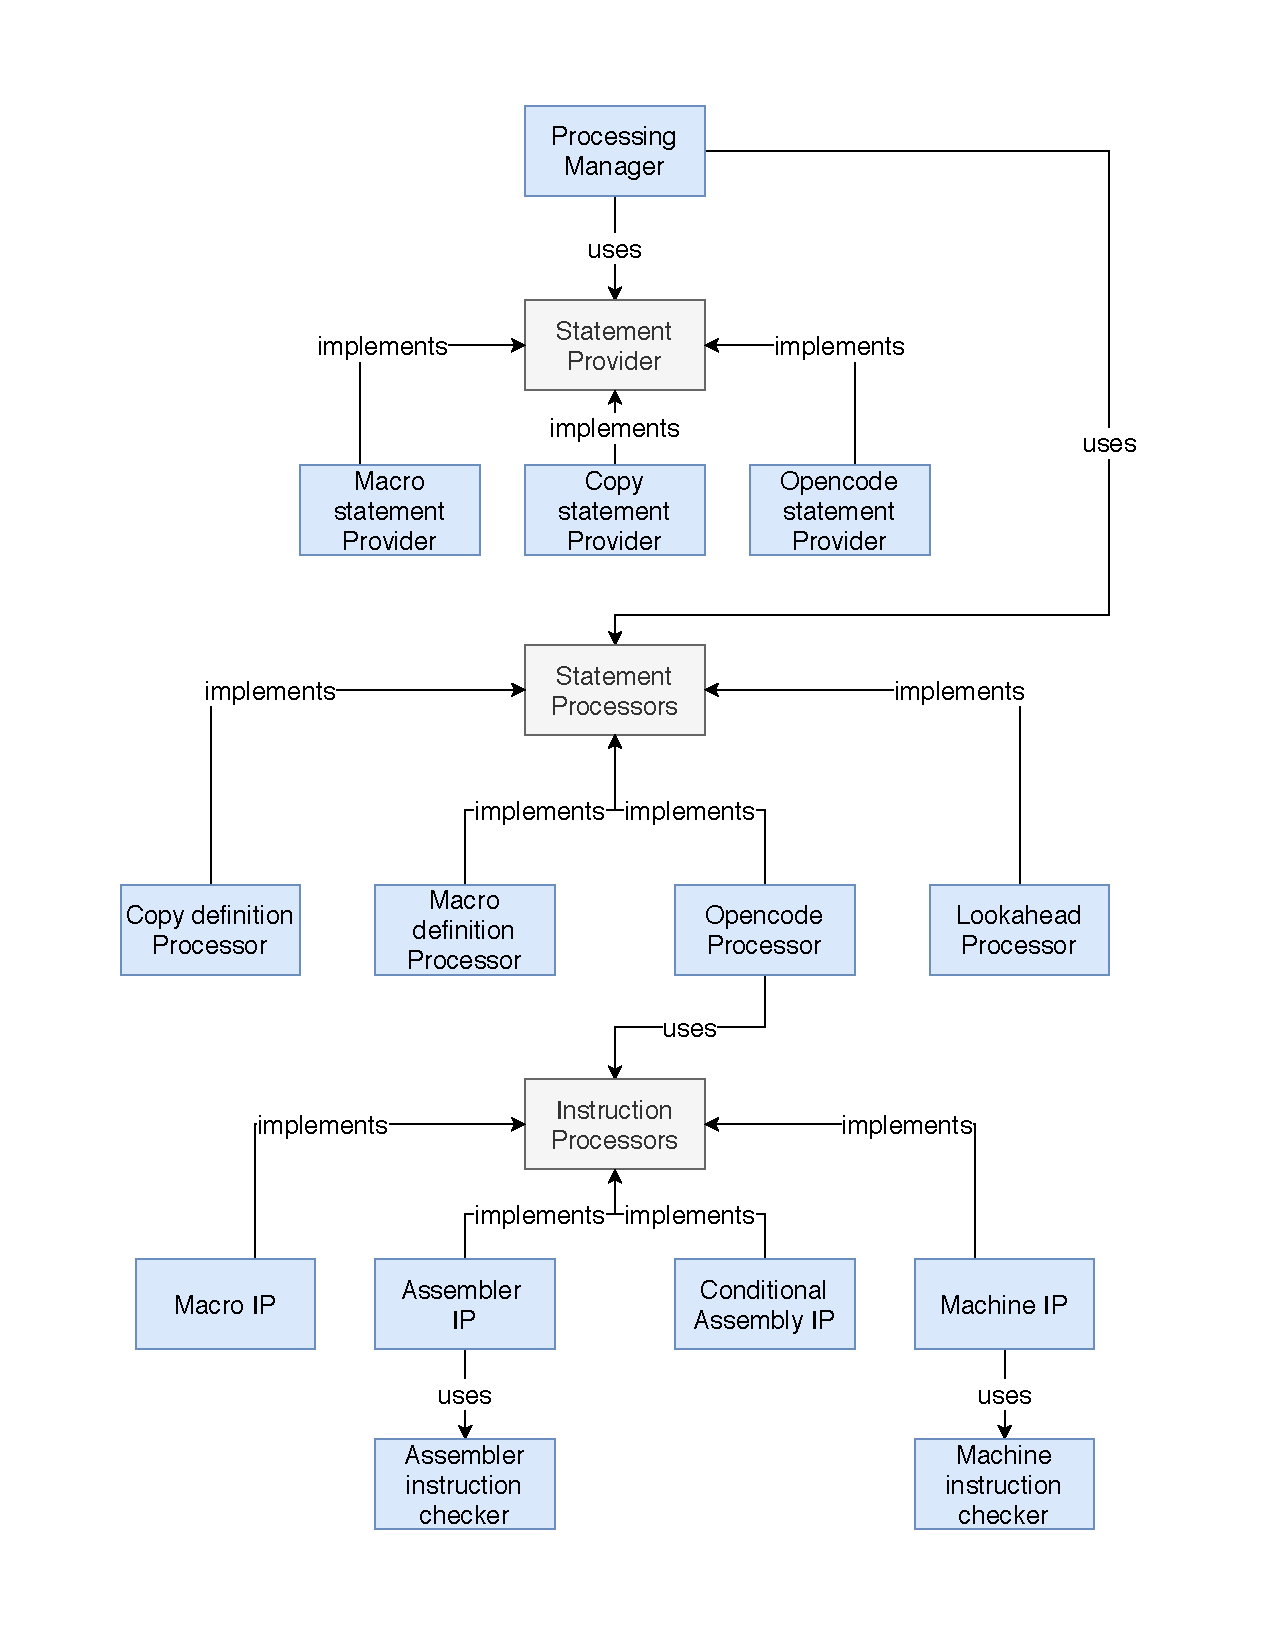
\includegraphics[width=\textwidth]{img/processing_manager_arch}
	\caption{The architecture of Processing manager}
	\label{fig06:proc_mngr}
\end{figure}

\subsection{Overview}

To construct processing manager, analyzer passes this objects to the constructor:
\begin{itemize}
	\item \emph{Parser} that provide statements from the processed file. Further on we will refer to the parser as to the \emph{Opencode statement provider}.
	\item \emph{HLASM context tables} that holds current state of the parsed source.
	\item \emph{Name} of the processed file.
	\item \emph{Library data} defining the initial state of the manager.
	\item \emph{Parse library provider} to solve in file dependencies.
	\item \emph{Statement fields parser} for parsing deferred statements (see ??). 
\end{itemize}

As the processing of the HLASM source file is rather complicated, we defined a \emph{statement provider} for each different source of statements and a \emph{statement processor} for each different manner of statement processing.

Processing manager captures this behavior. Hence, it contains two arrays, each consisting of different implementation of statement processor, or statement provider (see \cref{fig06:proc_mngr}).  Also, it has notion of the processor or provider that is in the current use and implement interfaces that change them.

\subsection{The main loop}

The main loop of the processing works with the current processor and provider. In the loop body, as the names suggest, statement provider provides next statement for statement processor that processes it accordingly. The loop breaks when the last processor finishes work.

However, the reader should focus on is when the current provider/processor is changed. The rules are:

\begin{enumerate}
	\item When the processor finished its work, the next processor is selected from the array.
	\item When the provider finished, before the next provider is selected from the array, manager checks whether the provider's end triggers finishing of the current processor as well (next refereed as \emph{terminal condition}). If true, performs rule 1.
\end{enumerate}

\subsection{Statement Providers}

In the processing manager, statement providers are stored in the array based on the priority (lower index, greater priority).

\begin{enumerate}
	\item Macro definition statement provider
	\item Copy definition statement provider
	\item Opencode statement provider
\end{enumerate}

Each cycle of the processor's main loop, providers are checked --- whether it has statements to provide --- based on the priority. That is because after each cycle, a processor with greater priority than the current one can be activated. 

For the main loop to be correctly defined, opencode provider's terminal condition holds for the all statement processors. Hence, when opencode provider finishes then all the processors finish as well and processing ends.

Let us explain the activation of respective providers:
\begin{itemize}
	\item Macro definition statement provider is activated when in source code, macro instruction is processed. Source of statements become the definition of the visited macro.
	\item Copy definition statement provider, similar to the provider above, is activated when copy instruction is processed. Source of statements become the definition of the copied source.
	\item Opencode statement provider is active as long as there are statements in the source file.
\end{itemize}

\subsection{Statement Processors}

The motivation in distinguishing different statement providers was the complexity of the HLASM language. There are many cases when the same statements require different processing under different circumstance (e.g. COPY instruction in macro is handled differently than in opencode, or lookahead processor can process statements that would fail to be processed by opencode processor).

In contrast to statement providers, statement processors can not be assigned a priority nor can be statically organized in an array. Hence, they are dynamically assigned to the manager's array when needed and removed from the array when they finish.

Each processor is responsible for the following:
\begin{enumerate}
	\item \emph{Copy definition processor} comes to effect when a source is copied to the processed file for the first time. It checks whether the copy definition comforts the rules and whether is well formed. When the processor processes whole definition it stores it in the HLASM context tables.
	\item \emph{Macro definition processor} is activated when a macro definition follows in a source file. It processes the prototype of the definition and checks for correctness of it. Then the created macro definition structure is stored in the HLASM context tables.
	\item \emph{Lookahead processor} activates when currently processed contitional assembly statement require value of the ordinary or sequence symbol that is not previously defined. It looks through following statements and finishes when the target symbol is found or when all the statement providers are exhausted.
	\item \emph{Opencode processor} is activated as a default processor in the source file processing. It checks and/or performs instruction statements with help of \emph{instruction processors}.
\end{enumerate}

\subsection{Manager's initial state}
Having described processors and providers, we are ready to talk about which of them are initialized by the manager at the beginning of the processing. The manager determines this by library data passed by analyzer.

Library data contains a file name and enumeration telling the meaning of the file that is being parsed --- \emph{processing kind}. 

\emph{Ordinary} processing kind states that the file being processed is the main source file (in HLASM jargon called open-code). It is the beginning processing file. With this information, manager initializes all the statement providers with respective order and \emph{only} opencode processor.

\emph{Copy} and \emph{Macro} processing kinds describe that manager will process file with copy or macro definition respectively. Hence, \emph{only} copy  definition processor (or macro definition processor respectively) is initialized.



\subsection{Expressions}
overview

they are parsed in grammar, later you give an expression "symbol evaluator" and it returns its value



\subsection{Data definition}

validation and processing purpose